\documentclass[a4paper,10pt]{article} %type de document et paramètres

\usepackage{lmodern} %police de caractère
\usepackage[english,french]{babel} %package de langues
\usepackage[utf8]{inputenc} %package fondamental
\usepackage[T1]{fontenc} %package fondamental

\usepackage[top=3cm, bottom=3cm, left=3cm, right=3cm]{geometry} %permet de paramétrer les marges par défaut
\usepackage{changepage} %permet de modifier localement une mise en page (marges,...) : utilisé pour la page de garde
\usepackage{multicol} %permet de mettre plusieurs colonnes (\begin{multicols}{2} \end{multicols} jusqu'à 10 colonnes)
\usepackage[pdftex, pdfauthor={Pierre Gimalac}, pdftitle={Activité bare-metal}, colorlinks=false, linkcolor=black]{hyperref} %permet de se déplacer dans le pdf depuis le sommaire en cliquant sur les titres, ainsi que de parametrer les meta données du PDF
\usepackage{url} %permet de mettre des URL actifs \url{}
\let\urlorig\url
\renewcommand{\url}[1]{\begin{otherlanguage}{english}\urlorig{#1}\end{otherlanguage}}

%\usepackage{mathtools} %maths (à developper, utile par exemple pour enlever les espaces dus aux boites $\sum_{\mathclap{1\le i\le j\le n}} X_{ij}$)
%\usepackage{amssymb} %maths
%\usepackage{amsthm} %maths
%\usepackage{amsmath} %maths
%\usepackage{mathrsfs} %maths (par exemple les lettres caligraphiées)
%\usepackage{stmaryrd} %maths (par exemple les ensembles d'entiers \rrbracket \llbracket)
%\usepackage{calrsfs} %maths (par exemple les notations des ensembles)
%\usepackage{yhmath} % permet de noter les arcs de cercle avec \wideparen{AOB}
%\usepackage{xlop} %permet d'afficher des opérations mathématiques
%\usepackage[squaren,Gray]{SIunits} %permet de noter des unités proprement
%\usepackage{esdiff} %permet d'écrire la dérivée avec la notation de Leibniz \diff{v}{t}

\usepackage{graphicx} %permet d'insérer des images proprement (ajoute des parametres)
\usepackage{wrapfig} %permet de mettre des images à coté d'un texte
%\usepackage{pdfpages} %permet d'insérer un pdf \includepdf[pages={1-2}]{truc.pdf}
\usepackage{enumitem} %permet de changer le label d'une liste \begin{itemize}[label=$\cdot$]
% \usepackage{ulem} %permet de souligner/barrer du texte
%\usepackage{soul} %permet de souligner/barrer du texte
% \usepackage{cancel} %permet de barrer du texte /cancel{text}
\usepackage{xcolor}

%\usepackage{tikz} %package trooop bien permet de dessiner tout et n'importe quoi ! \begin{tikzpicture}
%\usetikzlibrary{automata,positioning} % pour dessiner des automates
%\usepackage{circuitikz} %permet de dessiner des circuits logiques (entre autre) avec la syntaxe de tikz (\begin{circuitikz}) par exemple \node[american not port] pour le 'non'
\usepackage{listings} %permet d'inserer du code dans le fichier (\lstset{language=Java} \begin{lstlisting} \end{lstlisting} )
\usepackage{listingsutf8}

%\newcommand{\R}{\mathbb{R}}
%\newcommand{\Rpe}{\mathbb{R}_{+}^{*}}
%\newcommand{\Rb}{\overline{\mathbb{R}}}
%\newcommand{\N}{\mathbb{N}}
%\newcommand{\Z}{\mathbb{Z}}
%\newcommand{\C}{\mathbb{C}}
%\newcommand{\Q}{\mathbb{Q}}
%\newcommand{\K}{\mathbb{K}}
%\newcommand{\E}{\mathbb{E}} % espérance
%\renewcommand{\P}{\mathbb{P}} % fonction de probabilité
%\newcommand{\F}{\mathbb{F}}
%\newcommand\abs[1]{\left|#1\right|}
%\newcommand{\tq}{~|~}
%\newcommand\fra[2]{\genfrac{}{}{0pt}{1}{#1}{#2}}
%\newcommand\equi[1]{\renewcommand{\arraystretch}{0.3}~\begin{matrix}\sim\\#1\end{matrix}~\renewcommand{\arraystretch}{1}}
%\newcommand{\dl}{développement limité }
%\newcommand{\dls}{développements limités }
%\newcommand{\ev}{espace vectoriel }
%\newcommand{\evs}{espaces vectoriels }
%\newcommand{\sev}{sous-espace vectoriel }
%\newcommand{\sevs}{sous-espaces vectoriels }
%\newcommand{\displayAmath}{\displaystyle}
%\newcommand{\lime}[4]{#1\underset{\mathclap{#2 \rightarrow #3}}{\longrightarrow} #4}
%\newcommand{\supp}{\mathrm{supp}~} % support
%\newcommand{\Ima}{\mathrm{Im}~} % image
%\newcommand{\Inv}{\mathrm{Inv}~} % nombre d'inversion d'une permutation
%\newcommand{\ord}{\mathrm{ord}~} % ordre
%\newcommand{\com}{\mathrm{com}~} % comatrice
%\newcommand{\oversim}[1]{\overset{\sim}{#1}}
%\newcommand{\legendre}[2]{\left(\frac{#1}{#2}\right)}
%\newcommand{\Ber}{\mathrm{Ber}} % loi de Bernoulli

\lstdefinestyle{customc}{
  belowcaptionskip=1\baselineskip,
  breaklines=true,
  frame=L,
  xleftmargin=\parindent,
  language=C,
  showstringspaces=false,
  basicstyle=\footnotesize\ttfamily,
  keywordstyle=\bfseries\color{green!40!black},
  commentstyle=\itshape\color{purple!40!black},
  identifierstyle=\color{blue},
  stringstyle=\color{orange},
}

\lstset{language=C,style=customc,extendedchars=true,inputencoding=utf8,literate=
    {é}{{\'{e}}}1
    {è}{{\`{e}}}1
    {ê}{{\^{e}}}1
    {ë}{{\¨{e}}}1
    {û}{{\^{u}}}1
    {ù}{{\`{u}}}1
    {â}{{\^{a}}}1
    {à}{{\`{a}}}1
    {î}{{\^{i}}}1
    {ô}{{\^{o}}}1
    {ç}{{\c{c}}}1
    {Ç}{{\c{C}}}1
    {É}{{\'{E}}}1
    {Ê}{{\^{E}}}1
    {À}{{\`{A}}}1
    {Â}{{\^{A}}}1
    {Î}{{\^{I}}}1
}

\begin{document}

\LARGE
Activité bare-metal \hfill Télécom Robotics\\\\
\small Adressez toute faute, demande de précision ou d'ajout à Pierre Gimalac [\href{mailto:pierre.gimalac@gmail.com}{pierre.gimalac@gmail.com}]\\
ou directement sur le dépôt github [\href{https://github.com/TelecomParistoc/bare-metal-activity}{https://github.com/TelecomParistoc/bare-metal-activity}]

\normalsize
\renewcommand{\contentsname}{Sommaire}
\thispagestyle{empty}
\tableofcontents
\thispagestyle{empty}

\newpage

\section{Introduction}
L'objectif de cette activité est d'apprendre la programmation \textit{bare-metal}, c'est à dire sur microcontroleur, sans système d'exploitation pour nous faciliter la tâche.\\

En particulier il n'y a presque aucune abstraction avec le matériel à part celles fournies par le processeur, c'est à nous de charger le programme en mémoire et de gérer les interruptions.\\

De plus, il n'y a aucune fonction fournie et pas de gestion des processus donc tout doit se faire dans le même processus (dans un premier temps).\\

Une grosse partie de la programmation sur microcontroleur est de lire la documentation pour connaître le fonctionnement précis de celui-ci. Ce TP vous indiquera quels documents et quelles pages doivent être regardées pour vous éviter de lire des centaines de pages comme le pauvre auteur.\\

De plus, une architecture initiale est fournie pour éviter de passer trop de temps sans même arriver à exécuter un programme (voir \autoref{dependances} \nameref{dependances} et \autoref{fichiers_fournis} \nameref{fichiers_fournis}).\\

Le premier objectif du TP est d'arriver à allumer une LED située sur le microcontroleur en appuyant sur l'un des boutons.

\subsection{Que lire ?}
Ce TP est assez long, et il n'est pas \textit{obligatoire} de tout lire (mais je vous invite à le lire en entier tant qu'à faire), ci-dessous une liste d'un minimum à lire (parmi les sections \ref*{theorique}, \ref*{prerequis} et \ref*{fichiers_fournis}):
\begin{description}
\item[\nameref{gpio}] pour comprendre le TP
\item[\nameref{rules_config}] pour connaître les bonnes pratiques de programmation d'un microcontroleur
\item[\nameref{dependances}] pour pouvoir faire le TP
\item[\nameref{config}] pour pouvoir faire le TP
\item[\nameref{rappels_c}] pour arriver à écrire quoi que ce soit
\item[\nameref{bit_change}] pour configurer les registres
\item[\nameref{gdb}] pour flasher le programme sur le microcontroleur et le déboguer
\item[\nameref{documents}] qui décrit les fichiers de documentation fournis
\item[\nameref{include}] qui décrit les headers fournis, et comment les utiliser
\item[\nameref{makefile}] pour compiler le projet et lancer les différents programmes
\end{description}

Si vous faites le choix de ne lire que ces sections il se peut qu'il y ait des choses que vous ne compreniez pas, mais ça ne devrait pas vous empêcher de faire le TP.

\newpage

\section{\label{theorique}Quelques points théoriques}
\subsection{La mémoire des processus}
Chaque appareil dispose d'une quantité donnée de différents types de mémoire, en particulier des registres, de la mémoire vive (RAM) et de la mémoire morte (SSD, HDD).\\

Les exécutables sont composés de différents espaces de mémoire: text, rodata, data, bss et stack.

\begin{description}
    \item[text:] le code qui sera exécuté, certaines constantes
    \item[rodata:] les variables constantes (rodata = ``read-only data'')
    \item[data:] les variables modifiables
    \item[bss:] les variables initialisées à zéro (elles sont à part car cela fait gagner de la place)
    \item[stack:] la pile, l'espace de mémoire dynamique qui sert à stocker les variables locales et les informations lors des appels de fonction
\end{description}

Ci-dessous un tableau indiquant où est stocké chaque type de variable en C (voir \autoref{rappels_c} \nameref{rappels_c} si besoin).

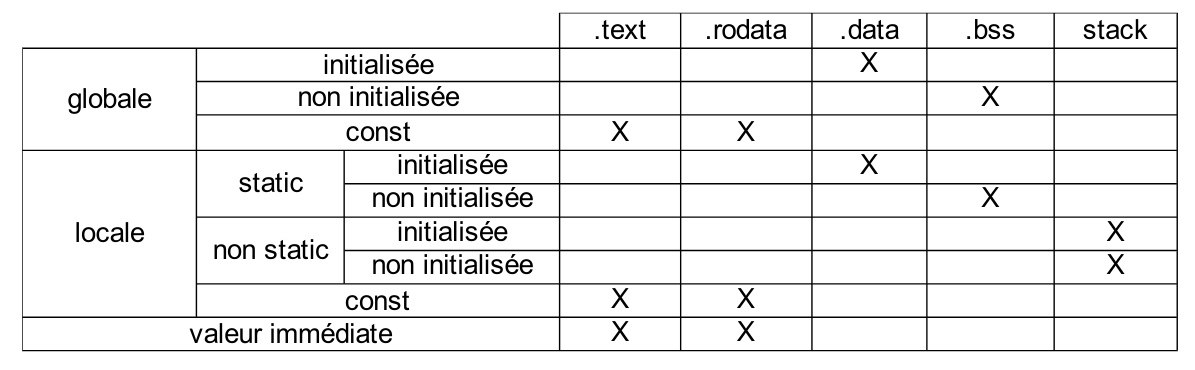
\includegraphics[scale=0.35]{assets/memory.png}

Le tas est un espace de mémoire dans lequel on peut allouer de la mémoire de taille variable et persistante (ne dépendant pas de l’exécution d'une fonction), il s'agit en fait d'une zone mémoire fournie par l'OS (sans trop rentrer dans les détails) donc que nous n'aborderons pas ici.

\subsection{Les périphériques}
Les périphériques sont ``mappés en mémoire'', c'est à dire qu'à chaque périphérique est associé un ensemble d'adresses virtuelles qui permettent de communiquer avec celui-ci.\\

Les documentations du périphérique et du microcontroleur indiquent quelles adresses sont à regarder et comment la communication et la configuration s'effectuent.

\subsection{\label{gpio}General Purpose Input Output}
Les General Purpose Input Output ou GPIO sont des moyens de communication génériques situés sur les microcontroleur. Leur avantage est d'être configurable de manière logicielle (et donc dynamique) en tant qu'entrée (un registre permet alors de lire la valeur), sortie (un registre permet alors d'écrire la valeur) ou même des fonctions alternatives spéciales.\\

Dans le cas qui nous intéresse, chaque GPIO dispose de 16 broches pouvant individuellement être programmées. Chaque GPIO possède des adresses virtuelles qui permettent de configurer ses broches de manière très précise. Il est même possible de générer des interruptions depuis des périphériques branchés sur une broche d'un GPIO.\\

La documentation indique les adresses de chacun des registres ainsi que la manière de les configurer.

\subsection{Les registres ARM}
\textit{Cette partie apporte des détails sur le fonctionnement des processeurs ARM mais n'est pas du tout nécessaire pour la réalisation du TP.}\\

Les processeurs ARM disposent de 16 registres\footnote{en vrai il y en a plus mais pas d'utilité courante}, ils sont appelés r0, r1, ..., r15.\\

Les registres r0 à r10 sont des registres d'utilité générale, c'est à dire que l'on peut les utiliser comme on veut.\\

Le registre r15 est aussi appelé Program Counter (PC), il pointe sur l'instruction que l'on est en train d’exécuter.\\
\begin{wrapfigure}{r}{8cm}
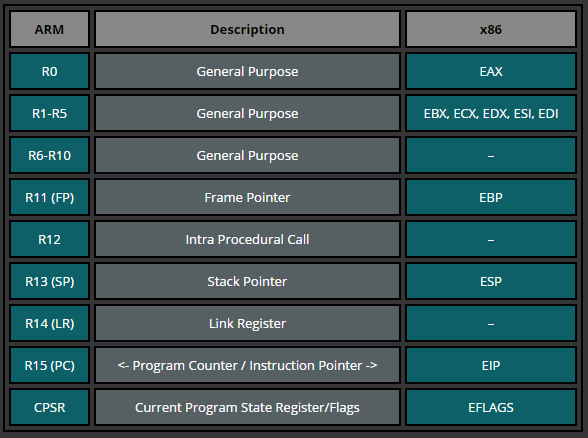
\includegraphics[scale=0.55]{assets/registers.png}
\end{wrapfigure}

Le registre r14 est le link register (LR), il contient l'adresse de retour lors de l'appel à une fonction.\\

Le registre r13 est le stack pointer (SP), il s'agit d'un pointeur vers l'extrémité de la pile.\\

Le registre r11 est le frame pointer (FP), il s'agit d'un pointeur vers le début de la zone de la pile attribuée à la fonction courante.\\

Ci-contre une comparaison avec les registres sous x86.\\

Lors d'un appel de fonction il faut savoir quels registres doivent être sauvegardés et par qui (fonction appelante ou fonction appelée), il s'agit d'une convention qui a des conséquences.

Dans le cas qui nous intéresse les registres r0 à r3 sont sauvegardées par l'appelant, ces registres vont contenir les paramètres des fonctions (s'il y a plus que 4 paramètres\footnote{ou que certains paramètres font 64 bits} on mettra les autres dans la pile). De plus le registre r0\footnote{r0 + r1 si on renvoie 64 bits} est utilisé pour stocker la valeur de retour.\\

Les registres r4 à r11 sont sauvegardés par la fonction appelée, cela évite de les sauvegarder s'ils ne sont pas utilisés, ils vont typiquement contenir les variables locales.\\

Le registre r12 n'est sauvegardé ni par la fonction appelée ni par l'appelante, il est donc utilisé de manière temporaire et il faut penser que chaque appel de fonction peut le modifier.

\subsection{\label{rules_config}Règle générale de configuration d'un microcontroleur}
La règle qui suit est presque toujours vraie (il y a donc des cas où on ne l'appliquera pas mais c'est rare): il ne faut modifier que les bits qui nous intéressent dans un registre, et laisser leur valeur aux autres pour éviter de créer des problèmes.\\

Pour voir comment modifier un bit particulier d'un registre, voir \autoref{bit_change} \nameref{bit_change}

\section{\label{prerequis}Prérequis}
\subsection{\label{dependances}Dépendances}
\begin{itemize}[label=$\bullet$]
    \item make
    \item toolchain arm-none-eabi
    \begin{itemize}
        \item sur ArchLinux:
        \begin{enumerate}
            \item arm-none-eabi-binutils
            \item arm-none-eabi-gcc
            \item arm-none-eabi-gdb
            \item arm-none-eabi-newlib
        \end{enumerate}
        \item sur Debian:
        \begin{enumerate}
            \item binutils-arm-none-eabi
            \item gcc-arm-none-eabi
            \item gdb-arm-none-eabi
            \item libnewlib-arm-none-eabi
        \end{enumerate}
    \end{itemize}
    \item JLinkGDBServer:
    \begin{itemize}
        \item Sur ArchLinux: jlink (AUR)
        \item Autre: débrouillez vous \href{https://www.segger.com/downloads/jlink/#J-LinkSoftwareAndDocumentationPack}{https://www.segger.com/downloads/jlink/}
    \end{itemize}
    \item latex (texlive) et pdflatex (pour compiler le sujet)
\end{itemize}

\subsection{\label{config}Configuration}
J'ai fait la configuration il y a plusieurs mois donc c'est compliqué de savoir quoi mettre ici.\\

Si vous rencontrez des erreurs ou des comportements étranges, signalez-le.\\

Pour pouvoir se connecter sur le microcontroleur sans être root il faut installer des règles udev, je crois qu'elles sont installées automatiquement sur ArchLinux mais je ne suis pas sûr de ce qui se passe avec d'autres OS.\\

Pour que GDB lise le .gdbinit fourni, il faut faire quelque chose dont je ne me rappelle pas, mais qui sera affiché la première fois que vous essaierez de lancer GDB (signalez-le à ce moment là).\\

Si vous êtes sur un autre Linux que Arch il faudra peut être modifier le Makefile pour donner le bon nom aux exécutables.

\subsection{\label{rappels_c}Langage C}
Si vous connaissez le langage C vous pouvez sauter cette section, il s'agit vraiment de points basiques pour que tout le monde puissent faire le TP.\\

Le langage C est ce que l'on appelle un langage bas niveau (comparativement à la plupart des langages modernes\footnote{demandez à Pierre Gimalac de vous parler du langage Rust}), ce qui signifie qu'il offre peu d'abstraction par rapport à l'assembleur et en particulier par rapport à l'utilisation de la mémoire.\\

\subsubsection{La syntaxe}
En première approximation sa syntaxe est proche de celle de Java:

\begin{multicols}{2}
\begin{lstlisting}[frame=single]
// déclaration de fonction
int sum(int a, int b) {
    return a + b;
}
\end{lstlisting}

\begin{lstlisting}[frame=single]
// boucle while
while (condition) {
    // do something
}
\end{lstlisting}

\begin{lstlisting}[frame=single]
// boucle for
for (int i = 0; i < 10; i++) {
    // do something
}
\end{lstlisting}

\begin{lstlisting}[frame=single]
// fonction main et appel de fonction
int main(int argc, char *argv[]) {
    return sum(-1, 1);
}
\end{lstlisting}

\begin{lstlisting}[frame=single]
// condition ternaire
long x = (y == 0 ? 0 : 1);
\end{lstlisting}

\begin{lstlisting}[frame=single]
// exécution conditionnelle
if (condition) {
    // do something
} else {
    // do something else
}
\end{lstlisting}

\begin{lstlisting}[frame=single]
// déclaration de tableau non initialise
int tab[10];
// déclaration de tableau avec contenu explicite
int tab2[] = { 1, 2, 3 };
\end{lstlisting}

\begin{lstlisting}[frame=single]
// opérations bit-a-bit
// et bit-à-bit
int x = a & b;
// ou bit-à-bit
int x = a | b;
// xor bit-à-bit
int x = a ^ b;
// non bit-à-bit
int x = ~a;
\end{lstlisting}

\end{multicols}

\subsubsection{Les types}
Les types primitifs en C sont\\

Pour les entiers:\\
- char, short, int, long, long long\\
- on peut rajouter unsigned devant (unsigned int) pour la version non signée\\

Pour les flottants:\\
- float, double, long double\\

Tous ces types ont des tailles différentes et variables selon les architectures.\\

Pour éviter ce piège potentiel, des types supplémentaires sont définis dans \textit{stdint.h}, qui sont int8\_t, int16\_t, int32\_t et int64\_t, la version non signée s'obtient en rajoutant un \textit{u} devant le type (uint32\_t). Le nombre correspond à la taille du type en bit. On utilisera ces types aussi souvent que possible, les seules exceptions sont le type char pour les chaînes de caractères et int qui correspond à la taille usuelle de calcul du processeur.\\

\bigskip

La partie délicate du C est en fait la partie qui diffère de Java. Il y a trois éléments sources de problèmes qui diffèrent de la syntaxe de Java.

\subsubsection{Préprocesseur}
Tout d'abord le préprocesseur, il s'agit d'un ensemble d'instructions qui seront exécutées à la compilation, et qui permettent de définir des valeurs et des fonctions, d'inclure des fichiers, ainsi que de faire des instructions conditionnelles.\\

Le préprocesseur remplace littéralement les occurrences des macros par leur définition.\\

\begin{lstlisting}[frame=single]
// on peut définir DEBUG depuis le fichier
// ou à la compilation en donnant le paramètre -DDEBUG à gcc
#define DEBUG
#include "file.h"
#ifdef DEBUG
    // en mode debug, LOG est une fonction qui affiche des messages sur la sortie erreur
    #define LOG(txt) printf(stderr, "%s\n", txt)
#else
    // hors mode debug LOG n'est pas défini et les appels a LOG disparaissent
    #define LOG(txt)
#endif
\end{lstlisting}

La directive \textit{\#define} remplace directement les occurrences du texte par la valeur. Ainsi un \textit{\#define VALUE 42} remplacera toutes les occurrences de \textit{VALUE} par la valeur 42.

\subsubsection{Gestion des fichiers multiples}
La gestion des fichiers se fait avec le préprocesseur et la commande ``include''.\\

Sans trop rentrer dans les détails sur le ``pourquoi'', pour chaque fichier \textit{.c} on définit un fichier \textit{.h} qui contient l'en-tête des fonctions que l'on veut exporter. On y met aussi les \textit{\#define} que l'on veut exporter, les structures et les directives préprocesseur \textit{\#include} qui sont nécessaires. On inclut ensuite le \textit{.h} dans le \textit{.c}, et tout se passe bien.\\

Pour éviter les problèmes d'inclusions mutuelles de fichiers (un fichier \textit{a.h} qui inclue un fichier \textit{b.h} et vice-versa), on rajoute une sécurité dans les fichiers \textit{.h}:

\begin{lstlisting}[frame=single]
// on choisit un nom qui sera unique à l'échelle d'un projet
// souvent on prend le nom du fichier auquel on rajoute un _H
#ifndef FILE_NAME_H
#define FILE_NAME_H

// ...
// contenu du fichier .h
// ...

#endif
\end{lstlisting}

\subsubsection{Pointeur}
On arrive enfin au cœur du sujet qui donne son nom de \textit{bas niveau} au langage C: les pointeurs et la gestion de la mémoire.\\

Les pointeurs sont un type de variable particulier, il s'agit d'une adresse mémoire qui pointe sur une valeur.\\

C'est plus compréhensible avec un exemple:

\begin{lstlisting}[frame=single]
int x = 42;
int *y = &x; // crée un pointeur vers x
int z = *y; // on déréférence y, ce qui récupère la valeur de x
\end{lstlisting}

y est ici un pointeur vers un entier (ce qui est indiqué par l'étoile dans le type \textit{int *}), le déréférencement de y \textit{*y} récupère la valeur pointée, donc celle de x.\\

Il faut faire attention: déréférencer un pointeur invalide (en particulier un pointeur nul) déclenche une erreur qui termine le programme.\\

Les avantages des pointeurs sont
\begin{itemize}
\item la taille fixe (32 ou 64 bits sur les plate-formes récentes), cela permet de passer un pointeur à la place d'une grosse structure, ce qui évite de grosses copies de mémoire
\item ils permettent de modifier des variables passées en argument, contournant ainsi la limite d'une seule valeur de retour
\item c'est grâce aux pointeurs que l'on utilise le tas et des buffers de taille variable\footnote{c'est également possible dans la pile mais de manière plus limitée}: la fonction malloc de la bibliothèque standard renvoie un pointeur vers une zone de mémoire de la taille demandée
\end{itemize}

\subsubsection{Volatile}
Le mot-clé volatile indique qu'une variable peut changer de valeur ``spontanément'', c'est-à-dire sans que le programme ne touche à la variable.\\

Le cas typique d'utilisation de ce mot-clé est pour les pointeurs sur des registres de périphériques.

\begin{lstlisting}[frame=single]
volatile uint32_t *reg = (volatile uint32_t *)0x40000800;
// reg est un pointeur vers un registre de 32 bits
// son adresse est 0x40000800
\end{lstlisting}

L'utilisation de volatile désactive certaines optimisations du compilateur, par exemple sans ce mot-clé deux lectures successives seraient transformées en une seule lecture. De même, pour deux écritures, ou pour des enchaînements de lectures et d'écritures.

\subsubsection{Petite précision sur les chaînes de caractères}
Les chaînes de caractères en C sont un peu particulières: une chaîne de caractères est un tableau de caractères qui termine par le caractère nul. Il faut faire attention de ne pas écrire après la limite du tableau (ce qui est techniquement tout à fait possible). Il faut également ne pas oublier le caractère nul à la fin sinon il est impossible de savoir quand arrêter de lire...

\subsection{\label{bit_change}Algèbre de Boole et opérations bit-à-bit en C}
Lorsque l'on paramètre un registre, on veut en général changer un bit (ou plusieurs) particulier et laisser les autres à leur valeur. Pour cela on doit utiliser des opérations bit-à-bit qui ne vont changer que ce que l'on veut changer.\\

Les opérations bit-à-bit disponibles sont:

\begin{tabular}{|c|c|c|l|}
\hline
nom & opérateur & nombre d'opérandes & description \\
\hline
et & \& & 2 & renvoie 1 si et seulement si les deux opérandes valent 1 \\
\hline
ou & | & 2 & renvoie 0 si et seulement si les deux opérandes valent 0 \\
\hline
xor & $\widehat{}$ & 2 & renvoie 1 si et seulement si une des deux opérandes vaut 1 \\
\hline
non & \texttildelow & 1 & renvoie 0 si l'opérande vaut 1 et inversement\\
\hline
left shift & $<<$ & 2 & décale les bits vers la gauche (indiqué par le 2e opérande) \\
\hline
right shift & $>>$ & 2 & décale les bits vers la droite (indiqué par le 2e opérande) \\
\hline
\end{tabular}

\subsubsection{Mettre un bit à 1}
Supposons que l'on ait une variable \textit{var} dont on veut mettre à 1 le 10e bit, sans toucher aux autres:

\begin{lstlisting}[frame=single]
// peu importe la valeur initiale de var
// on doit conserver tous ses bits,
// et mettre le 10e à 1
uint32_t var = 123456789;

var |= 1 << 10;
// 1 << 10 == 0b00000000000000000000010000000000
// on sait que 1 | 0 == 1 et 0 | 0 == 0 (le ou avec 0 conserve la valeur)
// donc le seul bit qui peut être modifié est le 10e
// il passe à 1, peu importe sa valeur initiale
\end{lstlisting}

\subsubsection{Mettre un bit à 0}
Supposons que l'on ait une variable \textit{var} dont on veut mettre à 0 le 10e bit, sans toucher aux autres. Celui là est un peu plus complexe que le précédent.

\begin{lstlisting}[frame=single]
// peu importe la valeur initiale de var
// on doit conserver tous ses bits,
// et mettre le 10e à 0
uint32_t var = 123456789;

var &= ~(1 << 10);
// 1 << 10 == 0b00000000000000000000010000000000
// ~(1 << 10) == 0b11111111111111111111101111111111
// on sait que 1 & 1 == 1 et 0 & 1 == 0 (le et avec 1 conserve la valeur)
// donc le seul bit qui peut être modifié est le 10e
// il passe à 0, peu importe sa valeur initiale
\end{lstlisting}

\subsubsection{Lire un bit}
Supposons que l'on ait une variable \textit{var} dont on veut lire le 10e bit.

\begin{lstlisting}[frame=single]
// on veut lire le 10e bit
uint32_t var = 123456789;

if (var & (1 << 10)) {
    // do something
}
// 1 << 10 == 0b00000000000000000000010000000000
// on sait que 1 & 1 == 1 et 0 & 1 == 0 (le et avec 1 conserve la valeur)
// donc le seul bit qui ne sera pas forcément à 0 est le 10e
// il garde sa valeur initiale

// donc var & (1 << 10) != 0 si et seulement si le 10e bit est à 1.
\end{lstlisting}

\subsubsection{Aide}
Pour éviter les problèmes sur les opérations bit-à-bit, des macros sont fournies:

\begin{lstlisting}[frame=single]
#define SET_BIT(REG, BIT) ((REG) |= (BIT))

#define CLEAR_BIT(REG, BIT) ((REG) &= ~(BIT))

#define READ_BIT(REG, BIT) ((REG) & (BIT))
\end{lstlisting}

Les noms et les définitions sont assez explicites, il est conseillé de les utiliser pour éviter les erreurs stupides. On fera attention au fait que le deuxième opérande BIT correspond à 1 $<<$ 10 dans nos exemples et pas juste à 10.

\subsection{La compilation du C}
La compilation du C est a priori moins facile que pour la plupart des autres langages: il n'y a pas de d'outil officiel pour compiler automatiquement et on a plusieurs types de fichiers sources et plusieurs types de fichier produits.\\

Cependant la compilation du C n'est pas si compliquée et la comprendre permet d'être beaucoup plus efficace quand on fait de gros projets.\\

La première étape de compilation est le préprocesseur, chaque directive include insert le code du fichier indiqué dans le fichier source, chaque define remplace le code en fonction de la définition. On peut demander à gcc\footnote{GNU C Compiler, le compilateur le plus utilisé pour le langage C} de ne faire que cette étape avec l'option -E.\\

L'étape suivante est la compilation du C vers l'assembleur par le compilateur. Les symboles inconnus (situés dans d'autres fichiers) ne sont pas résolus et on suppose qu'ils seront fournis plus tard. On demande à gcc de faire cette étape avec l'option S.\\

Ensuite, on génère un fichier binaire objet .o depuis le fichier assembleur. On a un fichier objet par fichier source (que ce soit c ou assembleur) On demande à gcc de faire cette étape avec le paramètre -c.\\

Enfin, on ``lie'' tous les fichiers objets entre eux (ainsi que les éventuelles bibliothèques utilisées) pour produire un unique binaire.\\

En général les fichiers intermédiaires (autres que les fichiers sources et les fichiers objets) sont supprimés. Il s'agit d'ailleurs du comportement par défaut de gcc (sans donner de paramètre particulier, gcc produit directement l’exécutable).\\

Cette méthode de compilation permet de ne recompiler un objet que si ses sources sont plus récentes, on évite ainsi pas mal d'opérations, ce principe est au cœur du fonctionnement des Makefile.

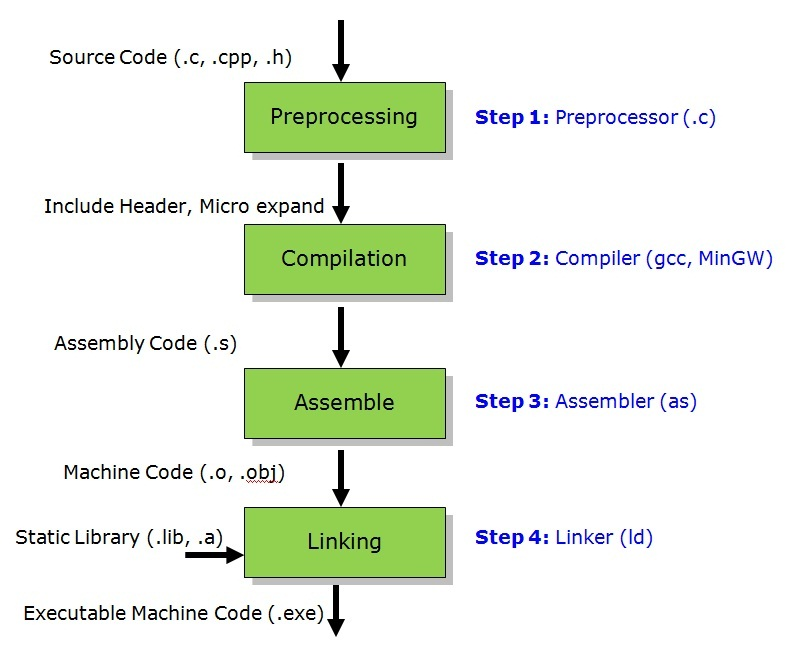
\includegraphics[scale=0.7]{assets/compilation.jpg}

\subsection{\label{gdb}How to debug: GDB}
Le GNU Debugger (GDB) est un outil très puissant qui permet de déboguer un programme en mettant des pauses dans l’exécution, en observant l'état de la mémoire (y compris des registres) et en exécutant instruction par instruction un programme.\\

Pour un meilleur débogage il faut compiler avec l'option -g, ce qui rajoute des infos de débug dans le binaire produit.\\

Les commandes principales sont
\begin{description}
    \item[b main.c:23] ajoute un breakpoint (une pause) à la ligne 23 du fichier main.c
    \item[c] reprend l’exécution d'un programme, attention dans le cas d'un microcontroleur on utilisera c pour lancer l’exécution du programme
    \item[run] lance l’exécution d'un programme (il est possible de donner des arguments à la commande run qui seront transmis au programme), ne pas utiliser sur un microcontroleur
    \item[mon reset] permet de reset le microcontroleur, ``mon'' indique que la commande est transmise au microcontroleur
    \item[load] charge le programme en mémoire
    \item[p var] affiche une variable
    \item[x var] affiche une variable en hexadécimal et le contenu de la case pointée (pratique pour un pointeur, sinon permet simplement d'avoir la valeur en hexadécimal)
\end{description}

\bigskip
Le fichier .gdbinit fourni contient quelques commandes pour vous faciliter la tâche et activer un meilleur affichage.

\begin{description}
    \item[flash] effectue un ``mon reset'' puis un ``load''
    \item[split] rajoute l'état des registres et le code assembleur dans la vue
    \item[ss] rajoute l'état des registres et le code C dans la vue
    \item[armex] commande pour déboguer en cas d'erreur, ça ne vous servira pas ici
\end{description}

Pour déboguer sur microcontroleur il faut lancer un serveur GDB qui fera le lien avec le microcontroleur et sur lequel GDB va se connecter ensuite (voir \autoref{makefile} \nameref{makefile} pour savoir comment le lancer).

\section{\label{fichiers_fournis}Les fichiers fournis}
\subsection{\label{documents}Documents}
Le dossier \textit{docs} contient la documentation nécessaire pour faire le TP, il y a trois documents: la datasheet des stm32f030, le manuel de référence des stm32f030 et le manuel utilisateur des stm32.\\

On vous indiquera dans quel document chercher chaque information à chaque étape.

\subsection{\label{include}Include}
Le dossier \textit{include} fournit des header C contenant beaucoup de macros très pratiques pour la programmation sur microcontroleur.\\

En particulier, il y a deux fichiers intéressants:
\begin{description}
    \item[stm32f030x8.h] contient les adresses de tous les registres de la doc, ainsi que des macros pour chaque bit de chaque registre et des bitmask. Il fournit également des types et des structures pour une utilisation plus lisible.

\begin{lstlisting}[frame=single]
// exemple d'utilisation
#include "stm32f030x8.h"

// GPIOA est une structure fournissant tous les registres du GPIOA
// GPIOA->BSRR est donc le registre BSRR du GPIOA

// Il y a une macro pour chaque bit et chaque masque
// Le format est comme ci-dessous, pour un registre lié aux GPIO
// ce sera GPIO_NOM_BIT (les noms sont les mêmes que dans la doc)
GPIOA->BSRR |= GPIO_BSRR_BS6;
\end{lstlisting}

Vous pouvez ouvrir le fichier et chercher dedans pour vérifier le nom des macros.

\item[stm32f0xx.h] contient des macros utiles pour interagir avec les registres (mentionnées dans la \autoref{bit_change} \nameref{bit_change})

\begin{lstlisting}[frame=single]
#define SET_BIT(REG, BIT) ((REG) |= (BIT))
#define CLEAR_BIT(REG, BIT) ((REG) &= ~(BIT))
#define READ_BIT(REG, BIT) ((REG) & (BIT))
#define CLEAR_REG(REG) ((REG) = (0x0))
#define WRITE_REG(REG, VAL) ((REG) = (VAL))
#define READ_REG(REG) ((REG))
#define MODIFY_REG(REG, CLEARMASK, SETMASK) \
    WRITE_REG((REG), (((READ_REG(REG)) & (~(CLEARMASK))) | (SETMASK)))
\end{lstlisting}

Il est conseillé d'utiliser intensivement les 3 premières et d'oublier les autres qui ne sont pas d'un grand intérêt.\\

Ce header importe également les sous headers en fonction du microcontroleur utilisé. Ici, il inclue donc le fichier ``stm32f030x8.h'' (pas besoin d'inclure les deux). Il suffit de définir STM32F030x8 (\textit{\#define STM32F030x8}) pour que cela fonctionne, et la définition est faite à l'échelle du projet dans le Makefile.\\

Ainsi un simple
\begin{lstlisting}[frame=none]
#include "stm32f0xx.h"
\end{lstlisting}
dans un fichier permet d'utiliser toutes les macros des deux fichiers.
\end{description}

\subsection{\label{makefile}Makefile}
Le Makefile est le fichier qui permet de compiler le projet de manière automatique et efficace: il contient des règles de construction de chaque fichier ainsi que des dépendances entre fichier, il ne reconstruit pas un fichier s'il est plus récent que sa source.

\subsubsection{Contenu}
Les premiers symboles définis sont des variables, les plus intéressantes / celles que vous pourriez vouloir modifier (ce n'est pas nécessaire mais vous pouvez expérimenter) sont:
\begin{description}
    \item[ASFLAGS] contient les paramètres de compilation des fichiers assembleur
    \item[CPPFLAGS] contient les paramètres du préprocesseur (on peut fournir des définition de macro à la compilation), on indique par exemple dans quels dossiers chercher les headers
    \item[CFLAGS] contient les paramètres de compilation des fichiers c, par exemple le flag -Ox indique le niveau d'optimisation (-O0 est stupide, -O3 fait des trucs incroyables)
    \item[LDFLAGS] contient les paramètres du linker
    \item[DIRS] est la liste des dossiers contenant des fichiers sources vous pouvez rajouter des dossiers
    \item[EXE] est le nom de l’exécutable (avec des extensions .elf et .bin selon ce que vous voulez)
\end{description}

Tout fonctionne de manière automatique: vous pouvez rajouter des fichiers .c ou .s (assembleur) dans n'importe quel dossier de DIRS et ils seront compilés et liés automatiquement.

\subsubsection{Utilisation}
La commande associée au Makefile est ``make''. Il faut faire ``make + \textit{nom de la règle}'' pour construire la règle voulue, et un simple ``make'' construit la première règle (qui est ici le fichier binaire).\\

\begin{description}
    \item[make] va construire le binaire
    \item[make gdb\_server] va lancer le serveur pour la connexion de gdb
    \item[make gdb] va lancer gdb et le connecter au serveur (donc faire make gdb\_server avant)
    \item[make tp] va produire le pdf de l'énoncé
    \item[make clean] va nettoyer les fichiers produits, sauf l’exécutable et le pdf de l'énoncé
    \item[make clean-all] va nettoyer tous les fichiers produits, y compris l’exécutable et le pdf
    \item[make re] fait ``make clean-all'' puis ``make''
\end{description}

Attention il faut se situer dans le dossier parent du TP (celui contenant le Makefile) pour utiliser toutes ces commandes.

\subsection{ld\_ram.lds}
Ce fichier indique au linker de quelle manière est organisée la mémoire du microcontroleur et de l’exécutable que l'on veut produire.\\

On peut voir les deux zones de mémoire (RAM et flash) avec leurs positions et tailles, ainsi que les différentes parties de l’exécutable et leurs positions en mémoire.

\subsection{lib/crt0.s}
Il s'agit du programme qui est exécuté initialement, on y définit une fonction \_start qui sera le point d'entrée dans le programme, on écrit dans le registre sp la valeur initiale de la pile, on appelle init\_bss qui initialise le bss (les variables initialisées à 0) et enfin on appelle la fonction main. On peut observer que l'on boucle indéfiniment à la fin.

\subsection{lib/init.c}
Ce fichier contient la fonction init\_bss qui initialise la bss (là où sont stockées les variables globales / static initialisées à 0) à 0.

\subsection{main.c}
Il s'agit du fichier principal, il contient la fonction main qui est (de votre point de vue) le point d'entrée du programme.

\section{Le vif du sujet}


\end{document}
